L'Andreu posa les nou boles que es mostren a continuació dins d'una bossa.
\begin{center}
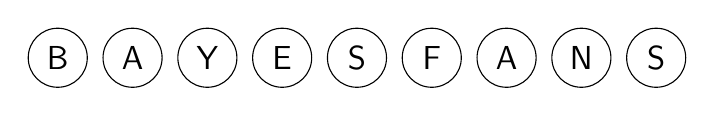
\begin{tikzpicture}
  \foreach \l [count=\i] in {B,A,Y,E,S,F,A,N,S}
    \node[draw,circle,minimum size=7.5mm,inner sep=0pt,font=\sffamily\large] at (0.95*\i,0) {\l};
\end{tikzpicture}
\end{center}

\begin{apartats}

\apartat{1,25}
A continuació, treu de la bossa dues boles a l'atzar, una darrere l'altra i sense reemplaçament (és a dir, no
retorna a la bossa la primera bola abans de treure la segona).
\begin{itemize}
\item[---] Calculeu la probabilitat que la primera bola sigui una A o una E. \emph{(0,5 punts)}
\item[---] Calculeu la probabilitat que les dues boles siguin diferents. \emph{(0,75 punts)}
\end{itemize}

\begin{solucio}
Com que hi ha dues A i una E, en la primera extracció tenim 3 casos favorables sobre 9 possibles; per tant,
la probabilitat demanada és $\frac39=\frac13$.\\
Calculem primer la probabilitat que les dues boles siguin iguals. Això només pot passar si són dues A o dues S:
\[
P(\text{dues A})=P(\text{primera A i segona A})=\frac29\cdot\frac18=\frac1{36}=P(\text{dues S}).
\]
Per tant, $P(\text{dues diferents})=1-P(\text{dues iguals})=1-2\cdot\frac1{36}=\frac{17}{18}=0{,}944\ldots$\\
Alternativament, podem argumentar directament de la manera següent: si la primera bola no és ni A ni S, segur
que les dues seran diferents; si la primera bola és una A, hi ha 7 boles favorables per a la segona extracció
(totes menys l'altra A); i, anàlogament, si la primera bola és una S, també hi ha 7 boles favorables per a la
segona extracció. Per tant,
\begin{align*}
P(\text{dues diferents})&=P(\text{primera no és ni A ni S})+P(\text{primera A i segona no A})\\
&\quad+P(\text{primera S i segona no S})=\frac59+\frac29\cdot\frac78+\frac29\cdot\frac78=\frac{17}{18}.
\end{align*}

\textit{Pauta oficial:} la primera pregunta, 0,5; la segona, 0,5 pel plantejament i 0,25 pel càlcul.
\end{solucio}

\apartat{1,25}
L'Andreu torna a posar totes les boles a la bossa i en treu cinc a l'atzar, una darrere l'altra, però ara amb
reemplaçament (és a dir, ara sí que retorna a la bossa cada bola extreta abans d'agafar la següent).
\begin{itemize}
\item[---] Calculeu la probabilitat que no hagi tret cap A. \emph{(0,5 punts)}
\item[---] Calculeu la probabilitat que hagi tret almenys dues A. \emph{(0,75 punts)}
\end{itemize}

\begin{solucio}
El nombre de boles A extretes segueix una llei binomial amb $n=5$ i $p=\frac29$.\\
$P(\text{cap A})=(1-p)^5=\left(\frac79\right)^5=0{,}284\ldots$\\
Passant al complementari, tenim
\[
P(\text{almenys 2 A})=1-P(\text{una A})-P(\text{cap A})=1-\binom51\left(\frac29\right)\left(\frac79\right)^4-\left(\frac79\right)^5
=0{,}308\ldots
\]

\textit{Pauta oficial:} la primera pregunta, 0,5; la segona, 0,5 pel plantejament i 0,25 per fer-ne el càlcul.
La segona pregunta es pot respondre també, de manera més llarga, calculant amb la binomial
$P(2\,\text{A})+P(3\,\text{A})+P(4\,\text{A})+P(5\,\text{A})$: doneu també aquestes respostes com a correctes en
la mesura que estiguin ben fetes i ben argumentades.
\end{solucio}

\end{apartats}
